\documentclass[tikz, preview]{standalone}

\usepackage{amsfonts, amsthm, amssymb, amsmath, stmaryrd, etoolbox}
\usepackage{tikz}
\usetikzlibrary{matrix,arrows}

\begin{document}
\[
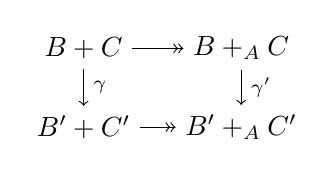
\begin{tikzpicture}
\node (BC) at (0,1) {$B+C$};
\node (BAC) at (2,1) {$B+_AC$};
\node (BC') at (0,0) {$B'+C'$};
\node (BAC') at (2,0) {$B'+_AC'$};
%
\draw [->>] (BC) edge (BAC);
\draw [font=\scriptsize,->] (BC) edge node[right] {$\gamma$} (BC');
\draw [font=\scriptsize,->] (BAC) edge node[right] {$\gamma'$} (BAC');
\draw [->>] (BC') edge (BAC');
\end{tikzpicture}
\]
\end{document}
